\section{Einleitung}
\label{s:intro}

Inhalt dieser wissenschaftlicher Arbeit ist das automatische Erstellen einer Material-Kostengliederung aus einer \ac{ifc}-Datei mit Hilfe von \ac{nlp} für eine Projekt einer Bausoftware. Die Bausoftware ist die ORCA AVA aus dem mittelständigen Softwarehaus \glqq ORCA Software GmbH\grqq{} aus Neubeuern. 
In diesem Kapitel soll eine kurze Einführung über die \glqq ORCA Software GmbH\grqq{} und das Produkt  ORCA AVA gegeben werden. Außerdem wird die Motivation für das Feature und die wissenschaftliche Vorgehensweise dieser Arbeit beschrieben.

\subsection{Ausgangssituation}
\label{c:intro:start}

Die im Titel beschriebene Bausoftware ist die ORCA AVA aus dem Softwarehaus \glqq ORCA Software GmbH\grqq{}. Dieses wurde im Jahr 1990 von Dipl.-Ing. Siegfried Tille und Dipl.-Ing. Heinz Nießen gegründet. Der Hauptsitz des Unternehmens ist in Neubeuern, bei Rosenheim. Das Unternehmen ist auf die Produktentwicklung von Software für die Baubranche spezialisiert. Im Vordergrund stehen die Ausschreibungssoftware ORCA AVA und die Ausschreibungstext-Plattform AUSSCHREIBEN.DE. Ziel der Entwicklung ist es die \ac{ava} eines Bauvorhabens für Planer, Architekten und Bauingenieure zu vereinfachen. Der Leitfaden ist, dass die Software soll für jeden verständlich und intuitiv zu bedienen sein.
Diese Arbeit fokussiert sich auf eine Erweiterung der ORCA AVA. Sie ist für alle Architektur- und
Ingenieurbüros, Wohnungsbaugesellschaften, Unternehmen und Behörden zur einfachen Abwicklung von Bauprojekten mit Ausschreibung, Vergabe und Abrechnung. Zusätzlich bildet sie das Kostenmanagement von solchen Projekten ab. Die Software ist außerdem \ac{bim} fähig und bietet \ac{din} zertifizierte Schnittstellen für den Datenaustausch an. Es stehen drei verschiedene Editionen zur Verfügung. Die ORCA AVA \ac{se}, die ORCA AVA \ac{pe} und die ORCA AVA \ac{ee}.  Die aktuellste Version ist die 25.0.

Technisch wird die ORCA AVA in .NET entwickelt. Ein Großteil der Anwendung besteht noch aus \ac{vb} Code. Alle neuen Komponenten und Erweiterungen werden in C\# implementiert. Neue \ac{gui}-Komponenten werden dementsprechend mit \ac{wpf} entwickelt. \ac{wpf} ist ein .NET Framework für das Erstellen von Windows Applikationen mit graphischer Benutzeroberfläche von Microsoft. \citep{Microsoft_2022} Die ORCA AVA und der IFC Manager (siehe Abschnitt \ref{s:basics:ifc:usage}) laufen in eigenen Prozessen und kommunizieren auf der Prozessebene auf der lokalen Umgebung. 

\subsection{Motivation}
\label{c:intro:motivation}


\ac{bim} bedeutet, dass die Planung von Bauprojekten vollständig auf digitaler Basis durchgeführt wird.  Für jeden Projektbeteiligten besteht somit Zugriff auf alle projektrelevanten Daten über Kosten, Mengen und Zeitabläufen. Somit können Baukosten einfacher ermittelt und der Bauprozess besser überwacht werden. In Abbildung \ref{fig:bim} ist zu sehen, dass \ac{bim} ein Relevanter Begriff in der Baubranche ist. Die Verwendung der Praktik ist allerdings noch nicht sehr verbreitet \citep[p.~20]{Thomas_Baumanns_Dr_Philipp-Stephan_Freber_Dr_Kai-Stefan_Schober_Dr_Florian_Kirchner2016-gu}. Mit dem \glqq \ac{ifc} First\grqq{} Ansatz ist das langfristige Ziel der ORCA AVA das Thema \ac{bim} noch mehr abzudecken. Die Ausschreibung soll automatisch aus dem 3D-Gebäudemodell entstehen. Bauteile aus dem Gebäudemodell sollen mit Kurztext, Langtext, Menge, Preis und vordefinierten Kostengliederungen in den Programmteil Bauelemente der ORCA AVA übernommen werden. Das ganze ist ein gutes Werbemittel für den Verkauf der Software, da die Relevanz des Themas so hoch ist und somit viele Kunden anspricht. Ein erster Teil des langfristigen Ziels, ist die Übernahme der Baustoffe aus der \ac{ifc}-Datei. Die Übernahme von weiteren Daten aus dem Gebäudemodell können darauf aufgebaut werden.
//todo: Kanomodell
\begin{figure}[h]
	\centering
	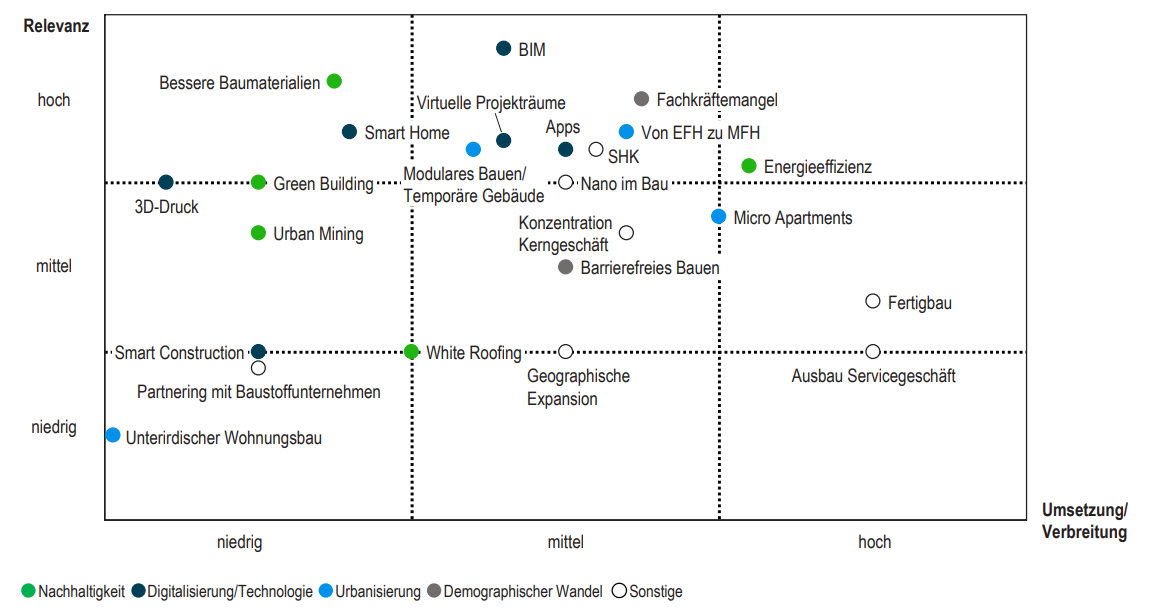
\includegraphics[scale=0.52]{bim-relevanz}
	\caption[Relevanz \ac{bim}]
	{Megatrends Nachhaltigkeit und Digitalisierung in der Bauwirtschaft. Bilder aus \citep[p.~20]{Thomas_Baumanns_Dr_Philipp-Stephan_Freber_Dr_Kai-Stefan_Schober_Dr_Florian_Kirchner2016-gu}}
	\label{fig:bim}
\end{figure}


Ein weiterer Trendbegriff, der mit dem Feature abgedeckt werden soll ist \glqq künstliche Intelligenz\grqq{} und \glqq Maschinelles Lernen\grqq{}. Das Suchinteresse der beiden Themen sind in Abbildung \ref{fig:ki-ml} zu sehen. Die Werte geben das Suchinteresse relativ zum höchsten Punkt im Diagramm an. Der Begriff \glqq Maschinelles Lernen\grqq{} hat seit Anfang 2015 eine steigendes Suchinteresse. Bei \glqq künstliche Intelligenz\grqq{} ist das Suchinteresse von Anfang 2017 bis Ende 2021 konstant hoch. Der starke Anstieg ab November 2022 hängt wahrscheinlich mit der Veröffentlichung der Software ChatGPT zusammen. Man erkennt das das Interesse über die letzten Jahre hoch ist.

\begin{figure}[h]
	\centering
	
	\begin{subfigure}{0.99\textwidth}
		\centering
	\includegraphics[width=1\linewidth]{künstiliche-intilligenz-trend}
		\caption{Suchinteresse: Künstliche Intelligenz}
		\label{FIG:ki-trend}
	\end{subfigure}
	\hspace{1cm}
	\begin{subfigure}{0.99\textwidth}
		\centering
	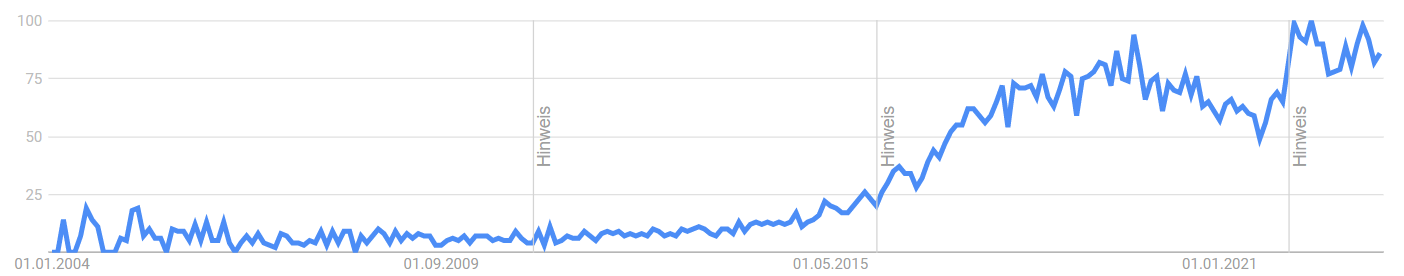
\includegraphics[width=1\linewidth]{machine-learning-trend}
		\caption{Suchinteresse: Machine Learning}
		\label{FIG:ml-trend}
	\end{subfigure}
	
	\caption[Google Trends]{Google Suchinteresse der beiden Begriffe \glqq künstliche Intelligenz\grqq{} und \glqq Maschinelles Lernen{} seit 2004}
	\label{fig:ki-ml-trend}
\end{figure}


\subsection{Methodik}
\label{c:intro:methodology}
\subsubsection{Wissenschaftliche Vorgehensweise}
\label{c:intro:methodology:scientific_proceture}
%\subsubsection{Zusatzinformationen Quellen}
%\label{ss:intro:methodology:sources}

\section{Grundlagen}
\label{s:basics}
In diesem Kapitel werden die Grundlagen im Bereich der Fachspezifischen Themen, Technik und Projektmanagement vermittelt. Dies sollte Verständnis für die folgenden Kapitel schaffen. Zuerst geht es um das Projektmanagement. Anschließend geht es um das Format \ac{ifc}, dessen Geschichte und dessen Nutzungsmöglichkeiten für diese Arbeit. Außerdem wird die Struktur und der Nutzen einer Kostengliederung in der ORCA AVA veranschaulicht.

\subsection{Projektmanagement}
\label{s:basics:project-management}
Bevor auf technische und fachliche Aspekte von \ac{ifc} und Kostengliederungen eingegangen wird, folgt die Einführung in das Projektmanagements mit SCRUM und \ac{devops}.

\subsubsection{Vorgehensmodell}
\label{s:basics:project-management:procedure_model}
Das Projekt wurde mit Hilfe agiler Softwareentwicklung durchgeführt. Die durchlaufenden Sprints sind zwei Wochen lang. Funktionale Anforderungen werden vom Projektmanagement gestellt.

\subsubsection{DevOps}
\label{s:basics:project-management:devops}
Die Bezeichnung \ac{devops} vereint die beiden Praktiken \glqq Development\grqq{}(Entwicklung) und \glqq Operations\grqq{}(Vorgänge). Die traditionelle Trennung von Entwicklung und Softwarebetrieb führt oft zu
Interessenskonflikten. Entwickler wollen stetig die Software verbessern, der Betrieb will Änderungen vermeinden um die Stabilität des Systems zu gewährleisten. Durch \ac{devops} entsteht ein Softwareentwicklungsprozess, den man durch Praktiken wie Continous Integration, Continous Delivery, Continous Deployment, automatisiertes Teste, Infrastructure-as-Code und automatische Veröffentlichungen beschleunigt. DevOps steht auch für eine Entwicklungskultur mit offener Zusammenarbeit, Kommunikation, Transparenz und Eingestehen von Fehlern, um Konflikte im Team zu vermeiden. Im Entwicklungsteam der ORCA AVA wird diese Praktik umgesetzt.
Die Technischen Hilfsmittel, die für den DevOps Prozess verwendet werden, sind in Abschnitt \ref{s:qs:technical_aids} \citep{devops_2021}

\subsection{IFC Format}
\label{s:basics:ifc}
Die Daten für die Material-Kostengliederung werden aus einem digitalem Gebäudemodel entnommen. Der öffentliche internationale Standard für Gebäudemodelle ist \ac{ifc}. \citep{BuildingSMART_International_Ltd2017-gs} Dieser wird auch in der bestehenden ORCA AVA benutzt um den Ausschreibungsprozess zu unterstützen. IFC Dateien können geöffnet, angeschaut und Informationen über das Modell in die Hauptsoftware übernommen werden.

\subsubsection{Verwendung}
\label{s:basics:ifc:usage}
Die ORCA AVA kann \ac{ifc}-Dateien einlesen. Im \ac{ifc} Manager wird das 3D-Modell dann angezeigt. In dem geöffneten Fenster gibt es dann einige fachliche Ansichten, die die \ac{ifc}-Daten nochmal abstrahieren. Es können bestimmte Mengen oder die Anzahl verschiedener Bauteile, die aus dem \ac{ifc}-Modell berechnet werden, in die ORCA AVA übernommen werden.
Es werden auch alle Eigenschaften eines Bauteils in der Eigenschaften-Ansicht angezeigt. Hier kann man auch die Materialbezeichnung des Bauteils finden, die im Modell hinterlegt ist.

Für das Arbeiten mit \ac{ifc}-Dateien wird die open-source Bibliothek xbim-toolkit verwendet. Die .NET Bibliothek kann \ac{ifc}-Dateien lesen, schreiben und anzeigen. Außerdem unterstützt es bei der Berechnung von komplexer Geometrie, um die Modelldaten für Analysen nutzbar zu machen. Seit 2009 wird das Projekt in Zusammenarbeit mit der Norhumbria Untiversity weiterentwickelt. Mittlerweile bildet es die Standards \ac{ifc2x3} und \ac{ifc4} zu 100\% ab. Außerdem bietet es an, auch \ac{ifc2x3} Modelle über das IFC4 Interface anzuprogrammieren. Somit können mit einer Codebasis beide Formate abgebildet und unterstützt werden. \citep{xbim}



\subsubsection{Geschichte}
\label{s:basics:ifc:history}
1994 startete die Entwicklung an dem offenen Datenmodellstandard \ac{ifc}. Dieser sollte die Anforderungen der Industrie an Interoperabilität gerecht werden und eine gemeinsame Basis zum Austausch von Informationen durch verschiedenen Anwendungen geschaffen werden. Mit \ac{bim} sollten Daten lesbar, editierbar für verschiedene Systeme durch den Bauprozess und kompletten Lebenszyklus eines Gebäudes geteilt werden. \citep{Laakso2012-oi}

\subsubsection{Dateiformat}
\label{s:basics:ifc:format}
IFC ist ein Implementierungs-Unabhängiges Datenmodell, welches in verschiedenen Umgebungen benutzt werden kann. Es kann beispielsweise in eine relationales Datenbankschema gegossen werden oder auch als Dateiformat implementiert werden. \citep{Laakso2012-oi}



\subsubsection{Baustoffe in IFC-Dateien}
\label{s:basics:ifc:buildingmaterial}
Das \ac{ifc} Modell bietet auch Materialangaben zu verschiedenen Bauteilen an. \citep{IFC4_doc}

\subsection{Möglichkeiten für die  Materialangabe eines Bauteils}
%\subsubsection{Material über LayerSet}
%\subsubsection{Material über MaterialList}
%\subsubsection{Material über ConstitutionSet}
%\subsubsection{Material über Material}
\subsection{Das Format Kostengliederung in der ORCA AVA}
\label{s:basics:coststructure}
Die Kostengliederung bietet eine Struktur, um Gesamtkosten einer Baumaßnahme in Kostengruppen unterteilt auswerten zu können. Logisch zusammengehörende Kosten können so in eine \ac{kg} zusammengerechnet werden. Außerdem ist der Aufbau eine Baumstruktur, wodurch Kostengruppen hierarchisch addiert werden können. 
Bei einem Bauprojekt kann man so Kosten über alle Projektphasen vergleichen. Von der Kostenschätzung über die  Ausschreibung bis zur Rechnungsfreigabe. So können Kostenauswertungen nach den verschiedenen Kostengruppen durchgeführt werden. In einem ORCA AVA Projekt kann man verschiedene Kostengliederungen definieren. Es existieren bereits Standardkostengliederungen beim Erstellen eines neuen Projektes. Zusätzlich können neue Kostengliederungen erstellt oder importiert werden.\citep{noauthor_undated-bx}

Technisch ist eine Kostengliederung als Modell im C\# Code definiert. Der Aufbau bildet die Baumstruktur über eine Referenz zur ParenNode und mehreren ChildrenNodes ab. Das Model kann dann über die ORCA AVA interne Middleware in der Datenbank persistiert werden. Die persistierten Kostengliederungen werden dann über VB-Teil der Anwendung im entsprechenden Programmteil angezeigt.
So müssen nach der generierten Kostengliederungs-Struktur die strukturierten Materialbezeichnungen in das C\# Modell abgebildet werden. So wird nach dem Import die erstellte Kostengliederung automatisch in der Oberfläche angezeigt und kann für Kostenauswertungen benutzt werden.

\section{Problemstellung und Anforderungen}
\label{s:requirements}
\subsection{Problemstellung}
\label{s:requirements:problem}
\subsection{Anforderungen}
\label{s:requirements:requirements}
\subsubsection{Funktionale Anforderungen}
\label{s:requirements:requirements:functional}
\subsubsection{Weitere Anforderungen}
\label{s:requirements:requirements:additional}
\subsubsection{Ziele}
\label{s:requirements:requirements:goals}

\section{Theoretische Konzeption für die Erstellung der Material-Kostengliederung}
\subsection{{Textklassifizierungsalgorithmus \dots}}
\subsection{{WordNet \dots}}
\subsection{\dots}

\section{Gegenüberstellung der möglichen Konzepte}
\subsection{Messkriterien}
\subsection{Vergleich der Konzepte}
\subsection{Festsetzten eines Algorithmus}
\section{Praktische Umsetzung}
\subsection{Zusammenfassen der Materialschnittstelle einer IFC Datei}
\subsubsection{Entwurf des Algorithmus}
\subsubsection{Implementieren des Algorithmus}

\subsection{Standardisierung der Materialnamen}
\subsubsection{Nutzen von Artificial Intelligence}

\subsubsection{Erstellen einer Datengrundlage}
\subsubsection{Implementierung der Standardisierung}

\subsection{Erstellen einer Kostengliederung}
\subsubsection{Implementieren}

\section{Maßnahmen zur Qualitätssicherung}
\label{s:qs}
\subsection{Clean Code}
\label{s:qs:cleancode}
\subsection{Technische Hilfsmittel}
\label{s:qs:technical_aids}
\subsection{Tests und Abnahme}
\label{s:qs:tests}
\section{Abschluss}
\label{s:closing}
\subsection{Bewertung der praktischen Umsetzung}
\label{s:closing:rating}
\subsection{Fazit}
\label{s:closing:conclusion}
\subsection{Ausblick}
\label{s:closing:outlook}
 Jo viel Spaß noch
